%% \listfiles
\documentclass[apj]{emulateapj}
%\documentclass[preprint2,12pt]{emulateapj}
%% \usepackage{natbib}
\usepackage{graphicx}
\usepackage{epsfig}
\usepackage{amssymb,amsmath}
\usepackage{array}
\usepackage{threeparttable}


\singlespace

%definitions
\newcommand{\Msol}{${\rm M_{\sun}}$}


%% Editing markup...
\usepackage{color}


%%%%%%%%%%%%%%%%%%%%%%%%%%%%%%%%%%%%%%%%%%%%%%%%%%%%%%%%%%%%%%%%%%%%%%%%%%%
% WARNING: This LaTeX block was generated automatically by authors.py
% Do not change by hand: your changes will be lost.

%%%%%%%%%%%%%%%%%%%%%%%%%%%%%%%%%%%%%%%%%%%%%%%%%%%%%%%%%%%%%%%%%%%%%%%%%%%


% --------------------- Ancillary information ---------------------
\shortauthors{SURP et al.}
\shorttitle{my short-title}
\slugcomment{Draft: \today}


\begin{document}

\title{This is the title}
 %% ---------
 
\author{SURP Students\altaffilmark{1}}
\altaffiltext{1}{CITA, University of Toronto}
 
\begin{abstract}
This is the abstract...
\end{abstract}

\keywords{cosmology: cosmic microwave background ---  gravitational lensing  }




\section{Introduction}
\label{sec:intro}

This is the introduction.


\section{Data}
\label{sec:data}
This is a section on Data. 
Here is an example of using the definitions above: a typical neutron star has a mass between $\sim$1.4 and 3.2 \Msol.


\subsection{Subsection 1}
\label{sec:cmb_data}
This is a sub-section.
Here is an equation:
\begin{equation}
E = mc^2
\label{eq:relativity}
\end{equation}
Here is an example of math-mode in the main text: $a^2 + b^2 = c^2$.  Here is a reference, to Fig.~\ref{fig:figureOfSpectrum}.  The data section is section \ref{sec:data}.


\begin{figure}
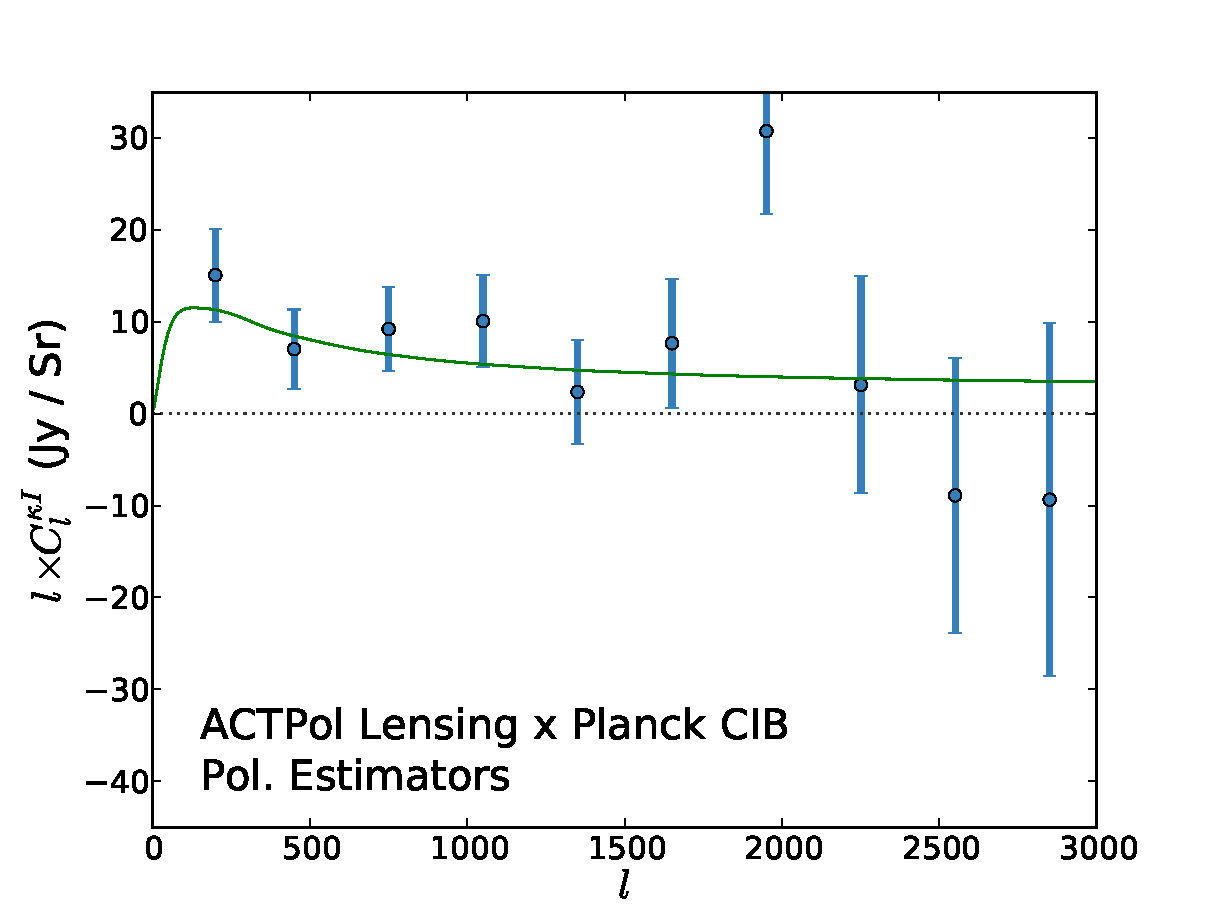
\includegraphics[width=1.05\columnwidth]{plotAllPatches_Polonly.pdf}
\caption{Here is how we insert a pdf figure.  This one is stolen from van Engelen+ 2014.\vspace{3mm}}
\label{fig:figureOfSpectrum}
\end{figure}



\begin{table}
\begin{center}
\begin{threeparttable}
\caption{A table.}
\begin{tabular}{|l|c|c|}
\hline 
Col 1 & Col 2 & Col 3 \\
 \hline  
Val 1 & Val 2 & Val 3 \\
Val 1 & Val 2 & Val 3 \\
\hline
\end{tabular} 
\vskip 2mm
\begin{tablenotes} \item  
\begin{center}
\begin{flushleft}
Description of table.
\end{flushleft}
\end{center}
\end{tablenotes}
\label{tab:vitalStats_kappa}
\end{threeparttable}
\end{center}
\end{table}


%\acknowledgments

%% %% \bibliographystyle{act}
%% \bibliographystyle{apj}

%% \bibliography{lenscib_refs.bib,apj-jour}



\end{document}
